\section{Dataset Construction}

In order to create this dataset, we collect a total of 204,659 book reviews from two online bookshops (Rokomari\footnote{\url{https://www.rokomari.com/}} and Wafilife\footnote{\url{https://www.wafilife.com/}}) using a web scraper developed with several Python libraries, including \verb|BeautifulSoup|, \verb|Selenium|, \verb|Pandas|, \verb|Openpyxl|, and \verb|Webdriver|, to collect and process the raw data.

% The data collection and preparation process that we follow for this dataset is a five-step process. First, we gather a list of URLs for books available on the aforementioned online bookshops. Next, we collect information about the books, including the names of the books and their authors, as well as the names of the categories they belong to and lists of reviews. In the third step, we collect the text of the reviews, along with ratings, reviewer names, and review dates. In the fourth step, we translate any English, Banglish (written with a combination of English and Bangla), or Romanized Bangla text into Bangla. Finally, in the fifth step, we label each review as positive, negative, or neutral based on ratings ranging from 1 to 5.
For the data collection and preparation process of the \textsc{BanglaBook} dataset, we first compile a list of URLs for authors from online bookstores. From there, we procure URLs for the books. We meticulously scrape information such as book titles, author names, book categories, review texts, reviewer names, review dates, and ratings by utilizing these book URLs. 
% We translate the review texts to Bangla and appropriately label them as positive, negative, or neutral.


\begin{table}[h]
 \centering
 \small
 \begin{tabular}{cc|c}
 \hline
 \parbox[t]{2mm}{\multirow{3}{*}{\rotatebox[origin=c]{90}{\begin{tabular}{c}\textbf{General} \\ \textbf{Properties}\end{tabular}}}} & \multicolumn{1}{c|}{\quad \# of Reviews} & \multicolumn{1}{c}{158,065}\\
 & \multicolumn{1}{c|}{\quad \# of Books} & \multicolumn{1}{c}{30,253}\\
 & \multicolumn{1}{c|}{\quad \# of Reviewers} & \multicolumn{1}{c}{44,616}\\
 & \multicolumn{1}{c|}{\quad \# of Categories} & \multicolumn{1}{c}{1,573}\\
 & \multicolumn{1}{c|}{\quad Total Review Words} & \multicolumn{1}{c}{44,429,201}\\
 \hline
 \parbox[t]{2mm}{\multirow{3}{*}{\rotatebox[origin=c]{90}{\begin{tabular}{@{}c@{}}\textbf{Single}\\ \textbf{Review}\end{tabular}}}} & \multicolumn{1}{c|}{\quad max. Word length} & \multicolumn{1}{c}{765}\\
 & \multicolumn{1}{c|}{\quad min. Word length} & \multicolumn{1}{c}{1}\\
 & \multicolumn{1}{c|}{\quad avg. Word length} & \multicolumn{1}{c}{281.08}\\
 \hline
 \end{tabular}
 \caption{General overview of \textsc{BanglaBook}.}
 \label{tab:tab2}
 \end{table}

 % \vspace{-10pt}



 
\subsection{Labeling \& Translation}
% If a review lacks a rating, it is deemed to be unannotated. 
If a review does not have a rating, we deem it unannotated. Reviews with a rating of 1 or 2 are classified as negative, a rating of 3 is considered neutral, and a rating of 4 or 5 is classified as positive. Two manual experiments are carried out to validate the use of ratings as a measure of sentiment in product reviews. In the first experiment, around 10\% of the reviews are randomly selected and annotated manually. The annotated labels are cross-checked with the original labels, resulting in a 96.7\% accuracy in the corresponding labels. In addition, we consult the work of \citet{Wang2020ARC} that explored the issue of incongruous sentiment expressions with regard to ratings. Specifically, the study scrutinized two categories of reviews: \textit{high ratings lacking a positive sentiment}, and \textit{low ratings lacking a negative sentiment}. We perform an analysis to identify such inconsistencies within our dataset and discovered that only a minuscule 3.41\% of the samples exhibited this pattern. This figure is relatively insignificant when considering the substantially large scale of our dataset.
 %%%%%%%%%%%%%%%%%%%%%%%%%%%%%%%%%%%%%%%%%%%%%%
\begin{figure}[h]
    \centering
    \subfloat[Sentiment Distribution\label{fig:donut_charta}]{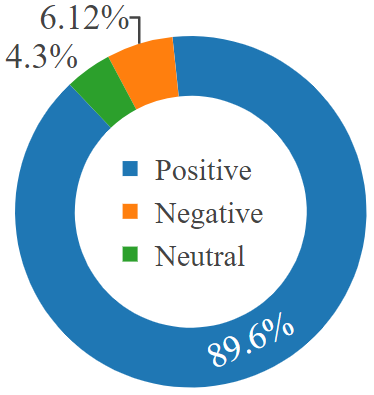
\includegraphics[scale=0.427]{images/ACLBookReview4.PNG}}\hspace{0.05cm}\subfloat[Rating Distribution\label{fig:donut_chartb}]{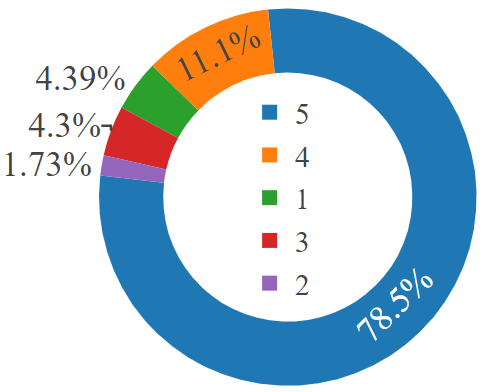
\includegraphics[scale=0.4]{images/ACLBookReview5.PNG}}
    % 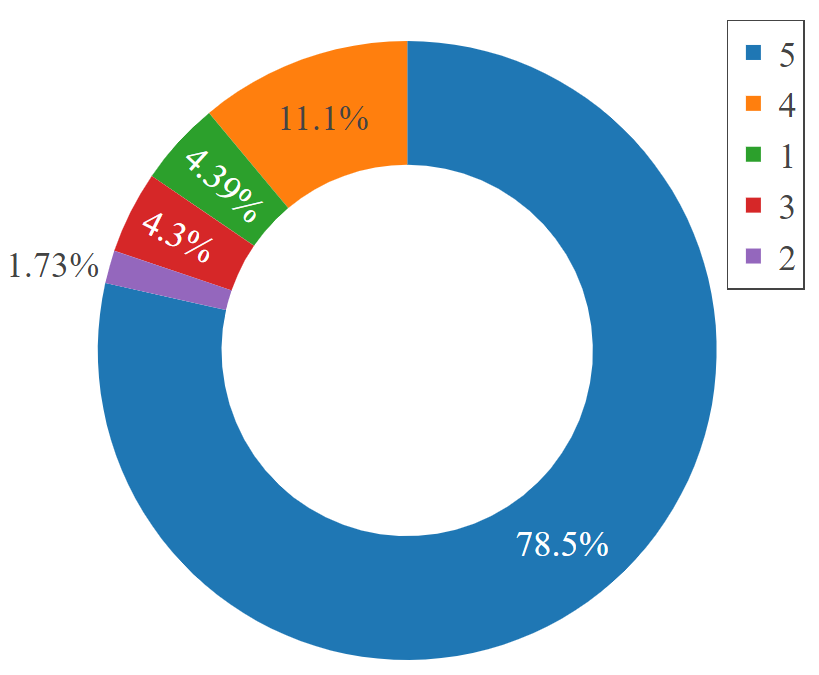
\includegraphics[scale=0.35]{images/ACLBookReview1.PNG}
    \vspace{10pt}
    \caption{Class Distribution of \textsc{BanglaBook}.}
    \label{fig:donut_chart}
\end{figure}
\\
%%%%%%%%%%%%%%%%%%%%%%%%%%%%%%%%%%%%%%%%%%%%%%
After discarding the unannotated reviews, we curate a final dataset of 158,065 annotated reviews. Of these, 89,371 are written entirely in Bangla. The remaining 68,694 reviews were written in Romanized Bangla, English, or a mix of languages. They are translated into Bangla with Google Translator and a custom Python program using the \verb|googletrans| library. The translations are subsequently subjected to manual review and scrutiny to confirm their accuracy. The majority of inaccurate translations primarily comprise spelling errors and instances where English words remain untranslated within samples containing a combination of Bangla and English text. The meticulous evaluation process of untranslated samples involves a thorough assessment by post-graduate native Bangla speakers, who critically compare the translated text against the original untranslated text to ascertain the correctness of the translation.
%%%%%%%%%%%%%%%%%%%%%%%%%%%%%%%%%%%%%%%%%%%%%%%%%%%%
\begin{table*}[htbp]
\centering
\scriptsize
 \begin{tabular}{p{8.0cm} P{1.1cm} P{1.1cm} P{1.1cm} P{2.0cm}} 
\toprule \textbf{Method} & \textbf{Negative}  & \textbf{Neutral}  & \textbf{Positive}  & \textbf{Weighted Avg.}  \\ \midrule
Random Forest{\fontfamily{qcr}\selectfont (word 2-gram + word 3-gram)} & 0.56 & 0.34 & 0.96 & 0.9106\\
SVM{\fontfamily{qcr}\selectfont (word 2-gram + word 3-gram)} & 0.40 & 0.15 & \textbf{1.00} & 0.9053\\
Random Forest{\fontfamily{qcr}\selectfont (word 1-gram)} & 0.48 & 0.35 & 0.96 & 0.9043\\
Logistic Regression{\fontfamily{qcr}\selectfont (char 2-gram + char 3-gram)} & 0.55 & 0.13 & 0.96 & 0.8978\\
Bangla-BERT{\fontfamily{qcr}\selectfont(base-uncased)} & 0.60 & 0.22 & 0.96 & 0.9064\\
Logistic Regression{\fontfamily{qcr}\selectfont (word 2-gram + word 3-gram)} & 0.53 & 0.13 & 0.96 & 0.8964\\
Bangla-BERT{\fontfamily{qcr}\selectfont (large)} & \textbf{0.72} & \textbf{0.40} & 0.97 & \textbf{0.9331}\\
\hdashline 
XGBoost{\fontfamily{qcr}\selectfont (char 2-gram + char 3-gram)} & 0.31 & 0.02 & 0.95 & 0.8723\\
Multinomial NB{\fontfamily{qcr}\selectfont (word 2-gram + word 3-gram)} & 0.23 & 0.03 & 0.95 & 0.8663\\
LSTM{\fontfamily{qcr}\selectfont (GloVe)} & 0.11 & 0.00 & 0.10 & 0.0991\\
XGBoost{\fontfamily{qcr}\selectfont (word 2-gram + word 3-gram)} & 0.23 & 0.01 & 0.95 & 0.8651\\
Multinomial NB{\fontfamily{qcr}\selectfont (BoW)} & 0.18 & 0.05 & 0.94 & 0.8564\\
SVM{\fontfamily{qcr}\selectfont (word 1-gram)} & 0.08 & 0.04 & 0.94 & 0.8519\\

\bottomrule
\end{tabular}
\caption{Catergory-wise Binary Task F1-score and Weighted Average F1-score of each method on \textsc{BanglaBook}.}\label{tab:baseline}
% \vspace{-10pt}
\end{table*}
%%%%%%%%%%%%%%%%%%%%%%%%%%%%%%%%%%%%%%%%%%%%%%%%%%%




%The translations are then manually inspected to ensure accuracy.

